% Results and Discussion Part Two: Hybrid descriptors enabled volcano plot for catalyst analysis


\section{Hybrid descriptors enabled volcano plot for catalyst analysis}

\begin{figure}
    \centering
    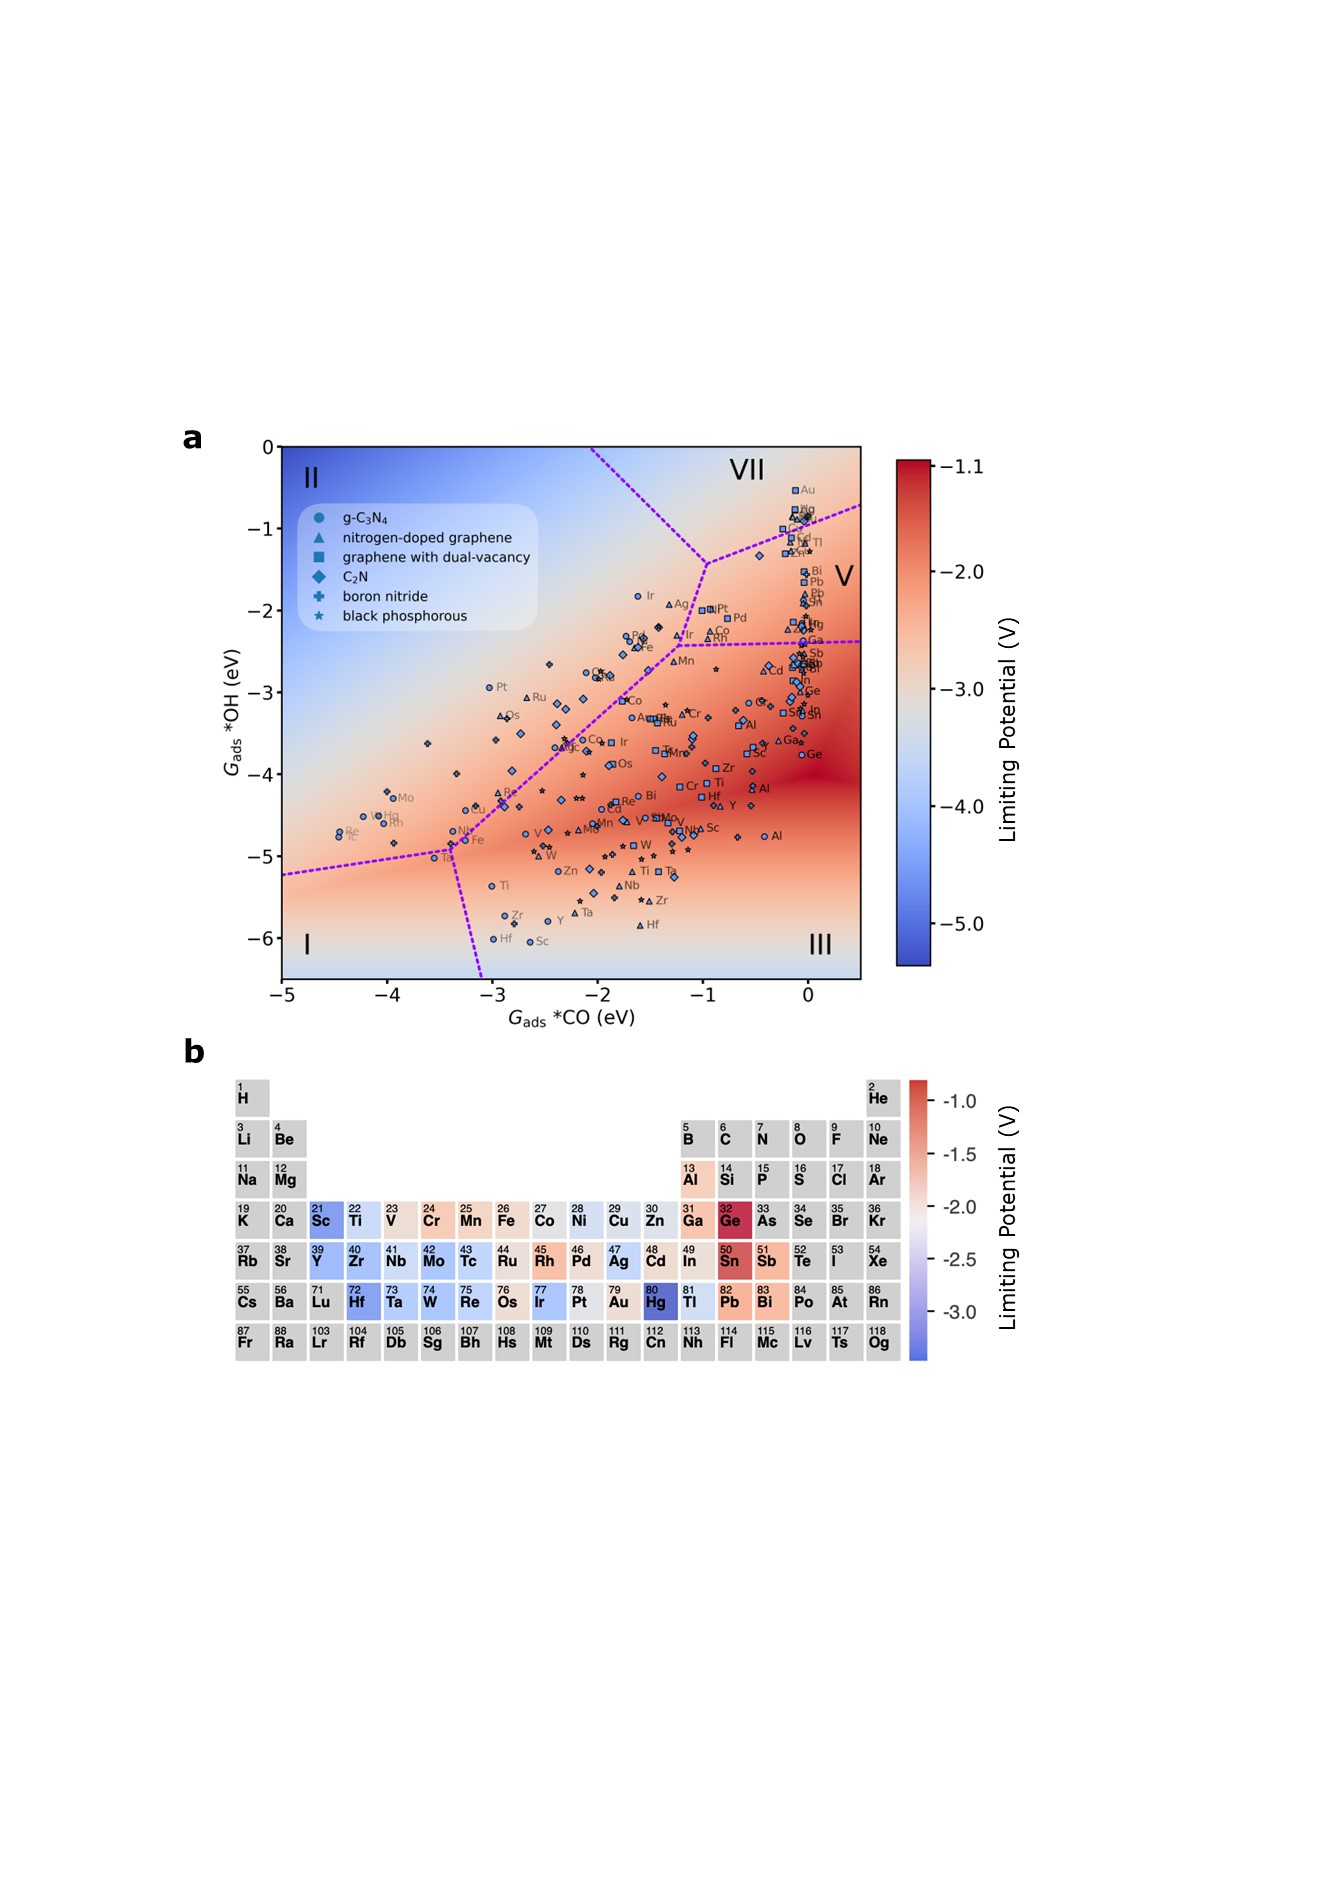
\includegraphics[width=0.95\linewidth]{main_sections/figures/figure_3.JPG}
    \caption{\textbf{Limiting Potential Volcano Plot and Periodic Table.}
    a. Limiting potential volcano plot computed from hybrid-descriptor-based linear scaling relations at -0.17 V vs SHE.
    In the plot, the circle, triangle, square, diamond, plus, and star symbols represent metals supported on g-$\mathrm{C_3N_4}$, nitrogen-doped graphene, graphene with dual-vacancy, black phosphorous, BN, and $\mathrm{C_2N}$, respectively.
    Dotted purple lines delineate regions representing rate-determining steps (RDS), with roman numerals denoting the respective RDS for each region.
    b. Limiting potential periodic table illustrating the theoretical activity of single atom catalysts, where metals are supported on g-$\mathrm{C_3N_4}$.}
    \label{main_fig3:volcano}
\end{figure}

Catalyst activity volcano plots, built upon the scaling relations proposed by Peterson and Nørskov's \cite{peterson2012activity},
goes beyond assessment of candidatures' energetics only but to provide informative guidance on discovering catalysts candidates with superior performance \cite{balandin1969modern, deutschmann2000heterogeneous}.
Our endeavor to improve the accuracy of volcano plots leads to the development of the hybrid-descriptor,
which encompasses both C- and O- bonding types of CO$_2$RR intermediates within the scaling relations.
This adaptation arose from the intuition that most CO$_2$RR intermediates are featured with both bonding types rather than any single one in dominance.
By integrating both bonding featured descriptors into the hybrid approach, we found the coefficient of determination ($R^2$) was increased by 0.1387.
Detailed information about the scaling parameters and performance enhancements are provided in Supplementary Tables 13 and Supplementary Figure 10.
This improvement to some extent underscored our premise that CO$_2$RR intermediates typically exhibit chemical similarities encompassing both O- and C-type descriptors.
After taking this dual nature into consideration, our hybrid-descriptor method can evaluate the intermediates adsorption energies more accurately.
Importantly, the introduction of hybrid descriptors is computationally affordable compared to DFT methods,
as it involves only a set of linear regressions to identify the optimal mixing ratio, as elaborated in the Methods section.

Expanding upon the revised scaling relations, we introduce an activity volcano plot and a rate-determining step (RDS) volcano plot for the CO$_2$RR process, shown in Figure 3a and Supplementary Figure 11.
Given that HER is a key competing reaction with CO$_2$RR \cite{goyal2020competition}, we also incorporated a selectivity volcano plot, presented in Supplementary Figure 12, to offer a comprehensive analysis of catalyst candidates.
In adherence to Peterson and Nørskov's original framework \cite{peterson2012activity}, our choice of x and y axes descriptors aligned with $\textit{G}_{\text{ads} \ast \text{CO}}$ and $\textit{G}_{\text{ads} \ast \text{OH}}$.
Further elaboration on how the limiting potentials were evaluated across the volcano plot can be found in the Methods section.
Among the candidatures explored, Ge@g-C3N4 emerged as the most promising catalyst, demonstrating theoretical activity at a limiting potential of -1.2126 eV.
Notably, the observed selectivity trend paralleled the activity trend, suggesting that catalysts exhibiting high theoretical activity are also resistant to HER side reactions.
The RDS volcano plot (Supplementary Figure 11) indicated protonation of *CO as the rate-determining step for nearly optimal candidates.
Moreover, the activity volcano plot predicted an optimal catalyst featuring a theoretical limiting potential of -1.0516 V, at $\textit{G}_{\text{ads} \ast \text{CO}}$ of 0.0589 eV and $\textit{G}_{\text{ads} \ast \text{OH}}$ of -4.0075 eV, positioned at the right-center of the volcano plot.
Results from RDS volcano plot indicate that protonation of *CO likely serves as the RDS for CO$_2$RR.
Consequently, it should be the focal point for future catalyst designs.
The activity and selectivity volcano plots imply that enhancing theoretical activity could be achieved by decreasing CO affinity while increasing OH affinity with the catalysts.
This result suggests a perspective: weak binding of CO to the catalyst surface might facilitate the rotation of C-O backbone from the “upright” configuration in *CO to the “horizontal” orientation in *CHO \cite{peterson2010copper},
and therefore facilitating dynamics and protonation of the *CO species.

The volcano plot offers an intuitive analysis of the reaction energetics and provides insights into the mechanisms of the reaction.
While the volcano plot provides a broad overview, it lacks the ability to delve into lower-level explanations rooted in electronic structures, where detailed electronic interactions and specific bonding mechanisms remain beyond its scope.
Despite its limitations, the volcano plot serves as a useful tool for identifying focal elementary steps in the reaction pathway that demand closer attention during catalyst design.
It also highlights directions for further catalyst refinement, and can also be integrated with the shifting experiment discussed later to optimize existing catalysts.

Additionally, we mapped the theoretical limiting potentials of the analyzed catalyst candidates onto periodic tables, shown in Figure 3b and Supplementary Figure 13 to 17.
Our analyses do not reveal consistent trends within groups or periods, nor did they exhibit evident patterns across substrates.
These observations suggest intricate interactions between supported metal atoms and substrates.
The absence of straightforward trends underscores the need for nuanced explorations in understanding these interactions like the CNN model.
